\label{sec:mva_lq}
Parametric Neural Networks (PNNs) are used as for the di-Higgs analysis to separate the signal from the expected backgrounds, and the PNN score distributions are final discriminant in the fit. Events are required to pass their respective selection criteria described in~\Cref{subsec:sellq_lephad},~\ref{subsec:sellq_hadhad} and the MC samples are weighted by their predicted cross sections.  The hyper parameters used for training used are summarised in~\Cref{tab:hyper_parameters_PNN_LQ}. In the~\Cref{sec:appendix_pnn}, studies on the input samples, hyper parameter optimization, signal statistics, and the over training checks are shown.

\FloatBarrier

\begin{table}
\centering
\small
\begin{tabular}{|c|c|}
\hline
Parameter & Value\\
\hline
Epochs & 100\\
Batch-size & 64\\
Learning rate & 0.1\\
Learning rate decay & 1e-5\\
Nesterov momentum & 0.9 \\
Layer sizes & 32 32 32\\
\hline
\end{tabular}
\caption{Training hyper parameters used for the LQLQ PNNs.}
\label{tab:hyper_parameters_PNN_LQ}
\end{table}

\subsubsection{\lephad}
The training is performed against the dominant \ttbar background with the real and fake tau components both taken from the MC simulation.
The input variables used to provide good discrimination between signal and background are:
\begin{itemize}
    \item $\Delta R(\ell,jet)$: the $\Delta R$ between the lepton and jet
    \item $\Delta \phi(\ell,E_{T}^{\mathrm{miss}})$: the opening angle between the light-lepton and the missing energy
    \item $s_{T}$ : the scalar sum of $E_{T}^{\mathrm{miss}}$, the $p_{T}$ of taus, two highest jets and lepton
    \item $E_{T}^{\mathrm{miss}} \phi$ centrality: the position in $\phi$ of $E_{T}^{\mathrm{miss}}$ between taus
    \item $m_{\tau,jet}$: the invariant mass between hadronic tau and its paired jet
    \item $m_{\ell,jet}$: the invariant mass between light-lepton and its paired jet
    \item \tauhad $p_T$
\end{itemize}

Input variable distributions are shown in Fig.~\ref{fig:PNN_input_lephad} for 1+2-$b$-tag signal region. The PNN score distributions
are shown in Fig.~\ref{fig:PNN_lephad}.

\begin{figure}
    \centering
    \subfloat[]{ \includegraphics[width=0.3\textwidth]{figures/mva/lq3/lephad/FinalPlots_TauLH_SR_cluster1_btag77_fullrun2_20210217_BasicKinematics_OS_combined_METCentrality_Rebin10.pdf}}
    \subfloat[]{ \includegraphics[width=0.3\textwidth]{figures/mva/lq3/lephad/FinalPlots_TauLH_SR_cluster1_btag77_fullrun2_20210217_BasicKinematics_OS_combined_m_LQ_had_Rebin25.pdf}}
    \subfloat[]{ \includegraphics[width=0.3\textwidth]{figures/mva/lq3/lephad/FinalPlots_TauLH_SR_cluster1_btag77_fullrun2_20210217_BasicKinematics_OS_combined_m_LQ_lep_Rebin25.pdf}}\\
    \subfloat[]{ \includegraphics[width=0.3\textwidth]{figures/mva/lq3/lephad/FinalPlots_TauLH_SR_cluster1_btag77_fullrun2_20210217_BasicKinematics_OS_combined_Tau0Pt_Rebin10.pdf}}
    \subfloat[]{ \includegraphics[width=0.3\textwidth]{figures/mva/lq3/lephad/FinalPlots_TauLH_SR_cluster1_btag77_fullrun2_20210217_BasicKinematics_OS_combined_dPhi_LepMET_Rebin15.pdf}}
    \subfloat[]{ \includegraphics[width=0.3\textwidth]{figures/mva/lq3/lephad/FinalPlots_TauLH_SR_cluster1_btag77_fullrun2_20210217_BasicKinematics_OS_combined_dR_J0Lep_Rebin20.pdf}}\\
    \subfloat[]{ \includegraphics[width=0.3\textwidth]{figures/mva/lq3/lephad/FinalPlots_TauLH_SR_cluster1_btag77_fullrun2_20210217_BasicKinematics_OS_combined_sT_Rebin40.pdf}}
    \caption{ 
     The pre-fit PNN input variable distributions in the LQLQ \lephad signal region. 
%     As discussed in the Sec~\ref{subsec:sellq_lephad}, these distributions include 1- and 2-$b$-tag events.
%     The red coloured line shows the LQ \lephad signal yields ($m=1100$ GeV).
    }
   \label{fig:PNN_input_lephad}
\end{figure}

\begin{figure}
    \centering
    \subfloat[]{ \includegraphics[width=0.3\textwidth]{figures/mva/lq3/lephad/Region_BMin0_incJet1_dist300_J2_Dbeta1p0PNN_T2_SpcTauLH_Y2015_LTT0_L1_Prefitlog.pdf}}
    \subfloat[]{ \includegraphics[width=0.3\textwidth]{figures/mva/lq3/lephad/Region_BMin0_incJet1_dist500_J2_Dbeta1p0PNN_T2_SpcTauLH_Y2015_LTT0_L1_Prefitlog.pdf}}
    \subfloat[]{ \includegraphics[width=0.3\textwidth]{figures/mva/lq3/lephad/Region_BMin0_incJet1_dist900_J2_Dbeta1p0PNN_T2_SpcTauLH_Y2015_LTT0_L1_Prefitlog.pdf}} \\
    \subfloat[]{ \includegraphics[width=0.3\textwidth]{figures/mva/lq3/lephad/Region_BMin0_incJet1_dist1000_J2_Dbeta1p0PNN_T2_SpcTauLH_Y2015_LTT0_L1_Prefitlog.pdf}}
    \subfloat[]{ \includegraphics[width=0.3\textwidth]{figures/mva/lq3/lephad/Region_BMin0_incJet1_dist1100_J2_Dbeta1p0PNN_T2_SpcTauLH_Y2015_LTT0_L1_Prefitlog.pdf}}
    \subfloat[]{ \includegraphics[width=0.3\textwidth]{figures/mva/lq3/lephad/Region_BMin0_incJet1_dist1200_J2_Dbeta1p0PNN_T2_SpcTauLH_Y2015_LTT0_L1_Prefitlog.pdf}} \\
    \subfloat[]{ \includegraphics[width=0.3\textwidth]{figures/mva/lq3/lephad/Region_BMin0_incJet1_dist1300_J2_Dbeta1p0PNN_T2_SpcTauLH_Y2015_LTT0_L1_Prefitlog.pdf}}
    \subfloat[]{ \includegraphics[width=0.3\textwidth]{figures/mva/lq3/lephad/Region_BMin0_incJet1_dist1400_J2_Dbeta1p0PNN_T2_SpcTauLH_Y2015_LTT0_L1_Prefitlog.pdf}}
    \subfloat[]{ \includegraphics[width=0.3\textwidth]{figures/mva/lq3/lephad/Region_BMin0_incJet1_dist1500_J2_Dbeta1p0PNN_T2_SpcTauLH_Y2015_LTT0_L1_Prefitlog.pdf}} \\

    \caption{ 
      The pre-fit PNN distributions in the LQLQ \lephad signal region.  
%     As discussed in the Sec~\ref{subsec:sellq_lephad}, these distributions include 1- and 2-$b$-tag events.
      The red coloured line shows the LQ \lephad signal yields for the corresponding mass point.
    }
         \label{fig:PNN_lephad}
\end{figure}

\subsubsection{\hadhad}
The training is performed against the dominant \ttbar background. The contribution of other backgrounds is small with respect to \ttbar events as shown in~\Cref{tab:LQHadHadYields}. The input variables chosen to provide a good discrimination between signal and background are:
\begin{itemize}
    \item $p_{T\tau 0}$: $p_T$ of the leading $\tau$
    \item ${\eta_{\tau 0}}$: $\eta$ of the leading $\tau$
    \item $m_{LQ0,1}$: the masses reconstructed from $b$ and $\tau$ which are paired by $\mathrm{min}|\Delta m|$ method described in~\Cref{subsec:btau_pairing}. The masses of both combination are used as input
    \item $\Delta R(\tau, jet)$: $\Delta R$ between the leading $\tau$ and the jet
    \item $E_{T}^{\mathrm{miss}} \phi$ centrality: the position in $\phi$ of $E_{T}^{\mathrm{miss}}$ between $\tau$'s
    \item $s_{T}$: the scalar sum of $E_{T}^{\mathrm{miss}}$, the $p_{T}$ of two $\tau$'s and two highest jets
\end{itemize}

Input variables distributions are shown in~\Cref{fig:PNN_input_hadhad}. The PNN score distributions are shown in~\Cref{fig:PNN_hadhad}.

\begin{figure}[]
    \centering
    \subfloat[]{ 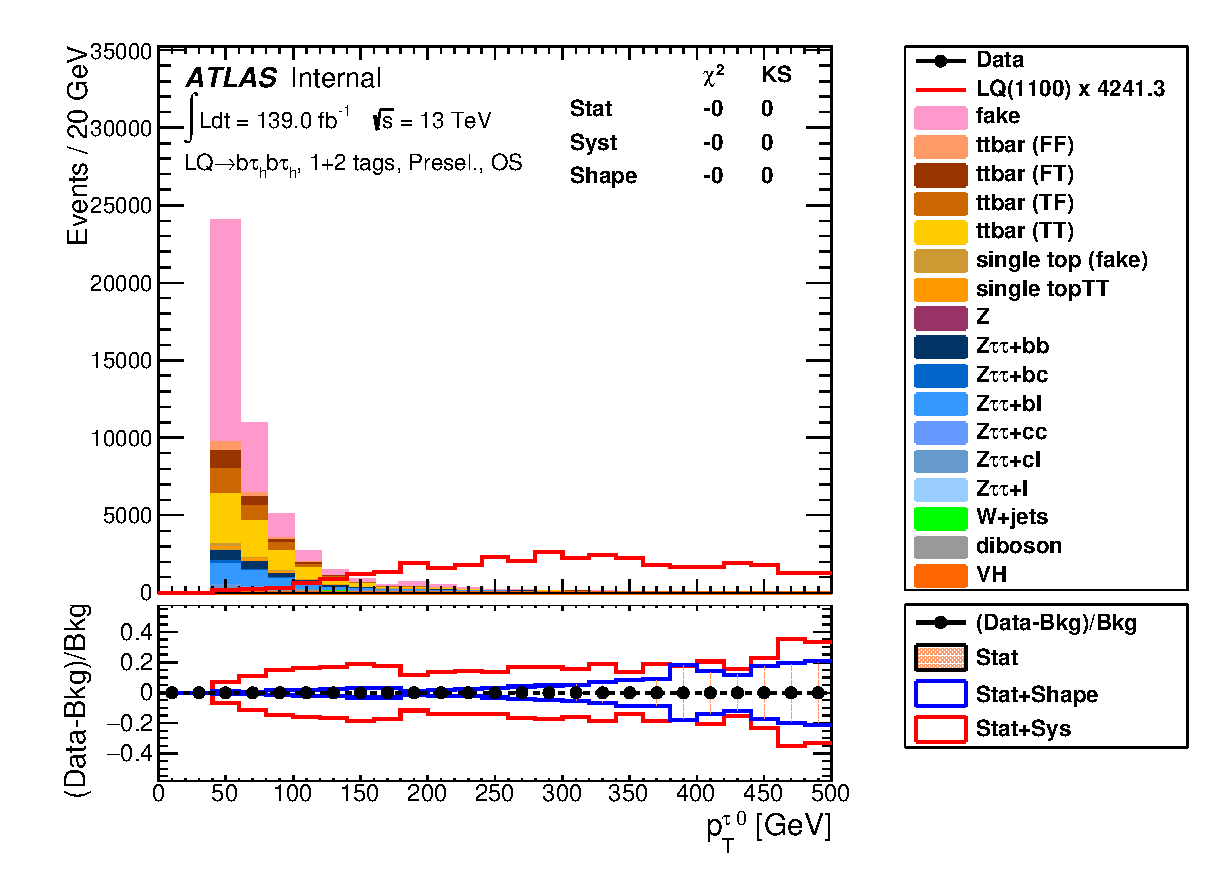
\includegraphics[width=0.4\textwidth]{figures/selection/lq3/hadhad/Plots_SR/C_3tag2pjet_0ptv_OS_Tau0Pt.eps}}
    \subfloat[]{ 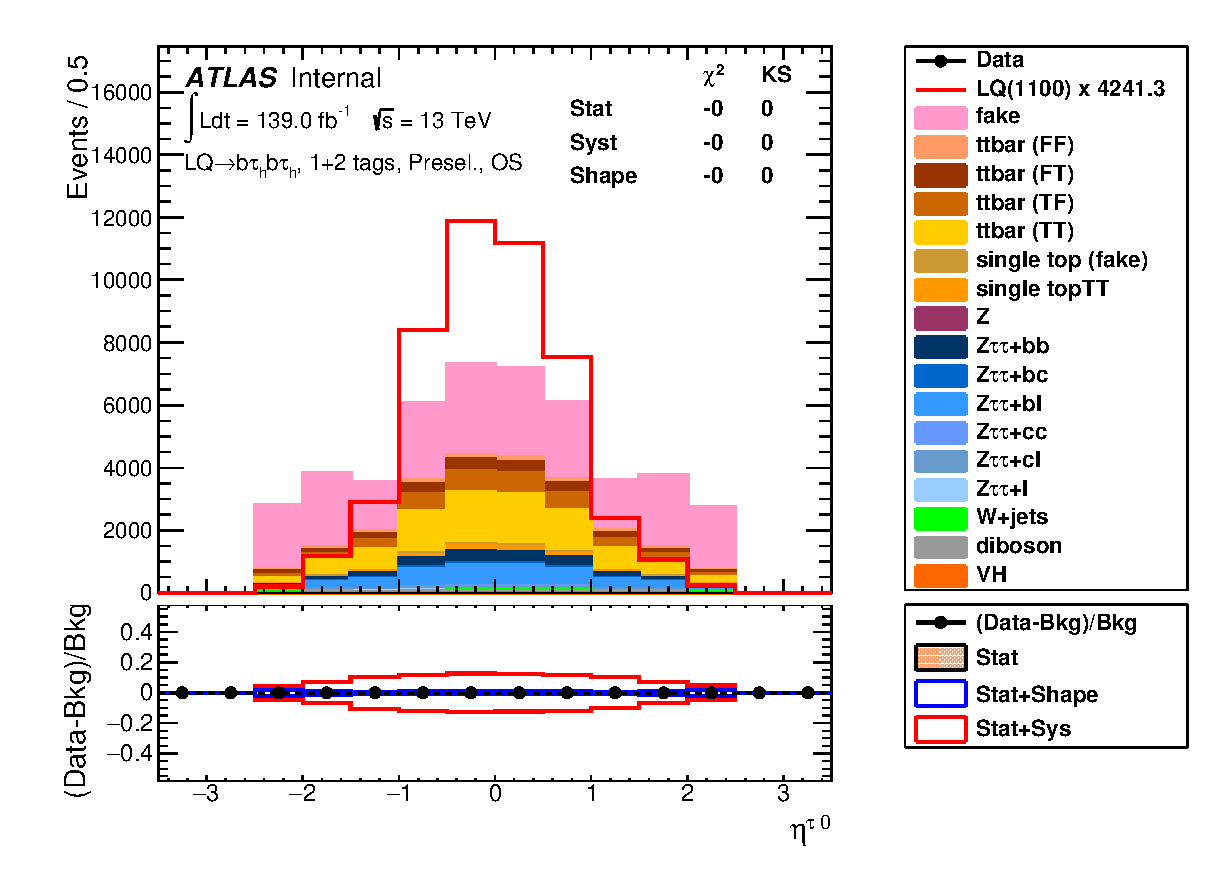
\includegraphics[width=0.4\textwidth]{figures/selection/lq3/hadhad/Plots_SR/C_3tag2pjet_0ptv_OS_Tau0Eta.eps}} \\
    \subfloat[]{ 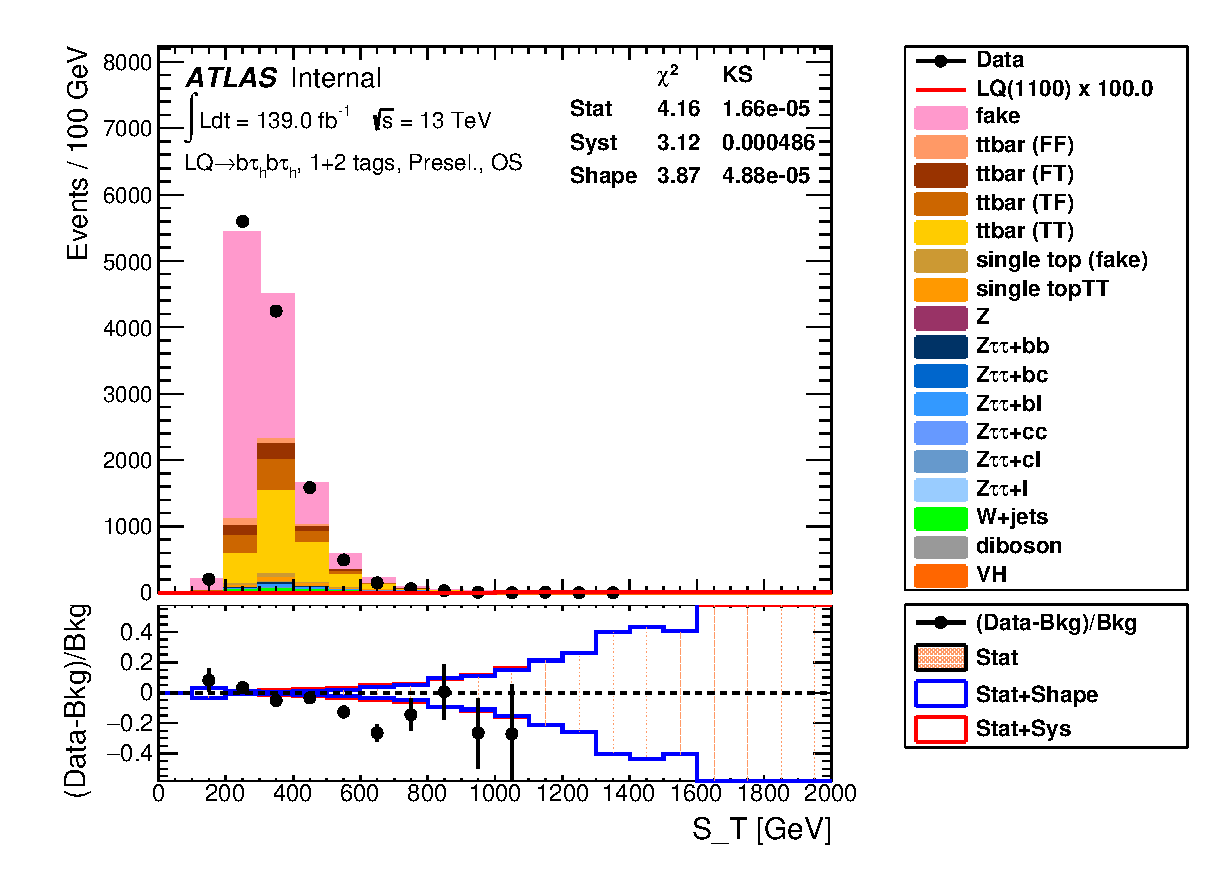
\includegraphics[width=0.4\textwidth]{figures/mva/lq3/hadhad/C_3tag2pjet_0ptv_OS_SR_sT.eps}}
    \subfloat[]{ 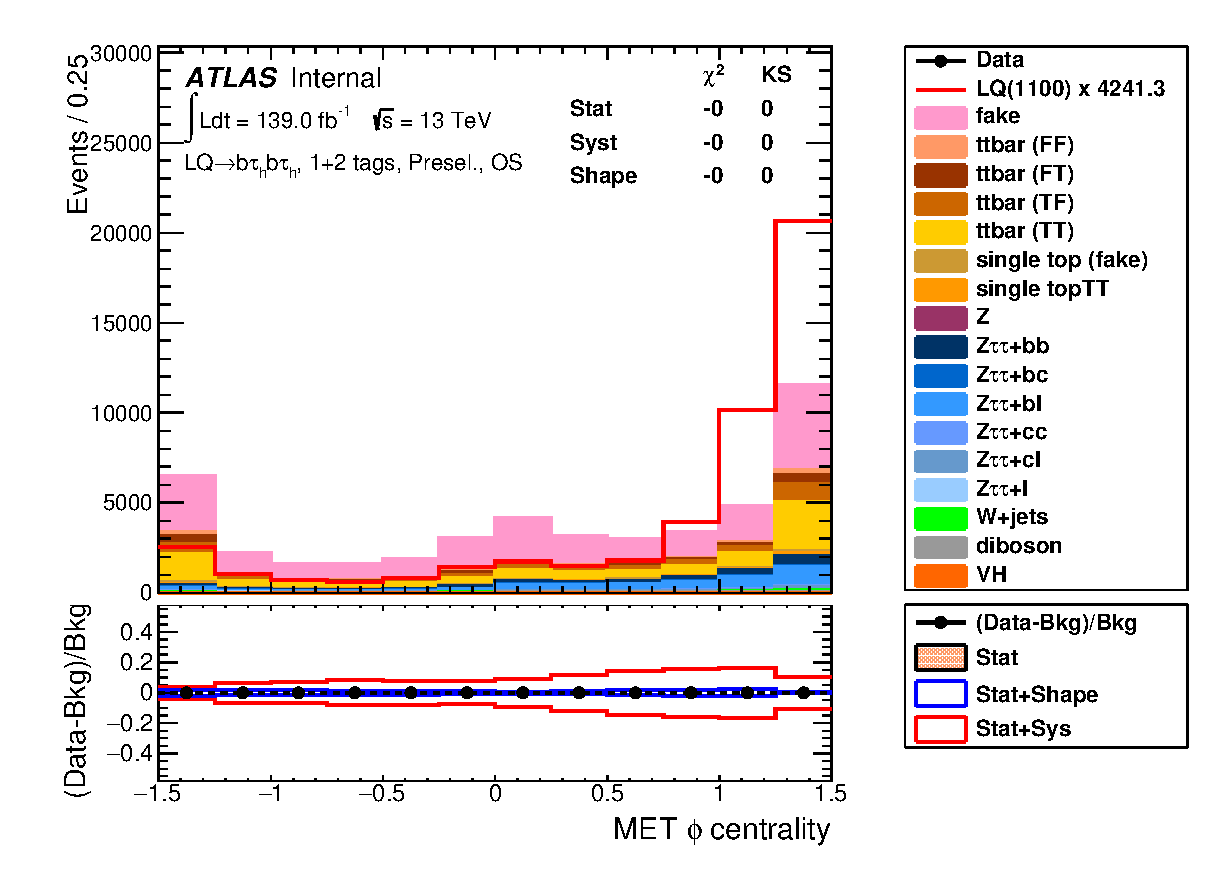
\includegraphics[width=0.4\textwidth]{figures/mva/lq3/hadhad/C_3tag2pjet_0ptv_OS_SR_METCent.eps}} \\
    \subfloat[]{ 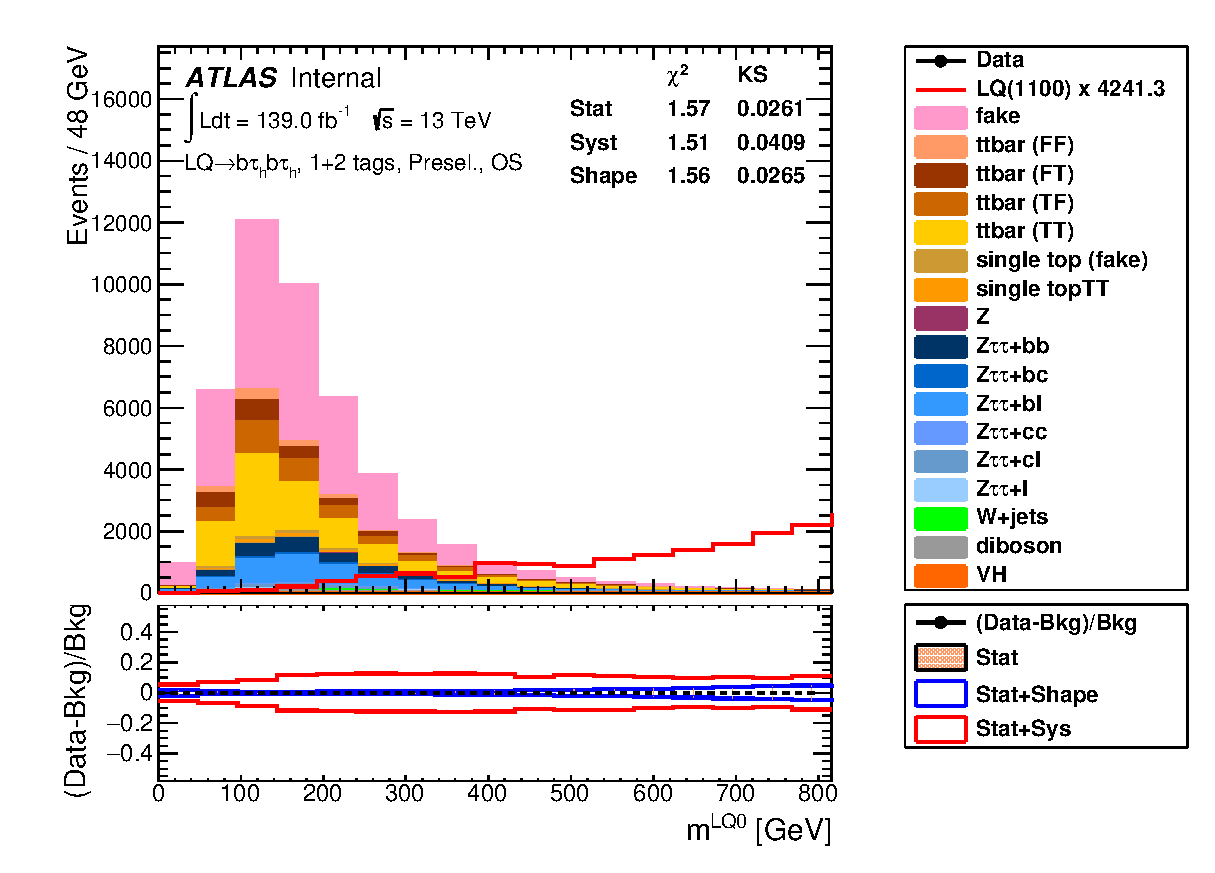
\includegraphics[width=0.4\textwidth]{figures/mva/lq3/hadhad/C_3tag2pjet_0ptv_OS_SR_m_LQ0.eps}} 
    \subfloat[]{ 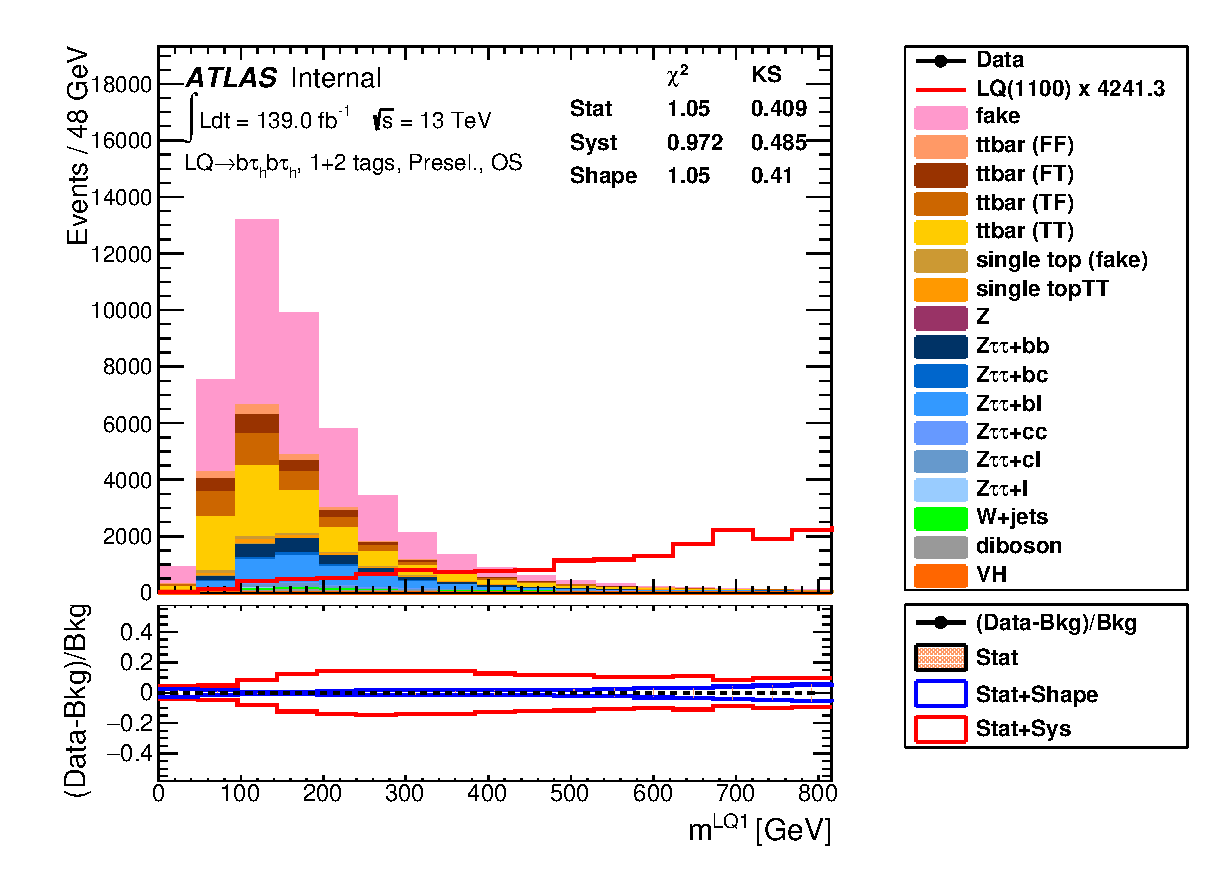
\includegraphics[width=0.4\textwidth]{figures/mva/lq3/hadhad/C_3tag2pjet_0ptv_OS_SR_m_LQ1.eps}} \\
    \subfloat[]{ 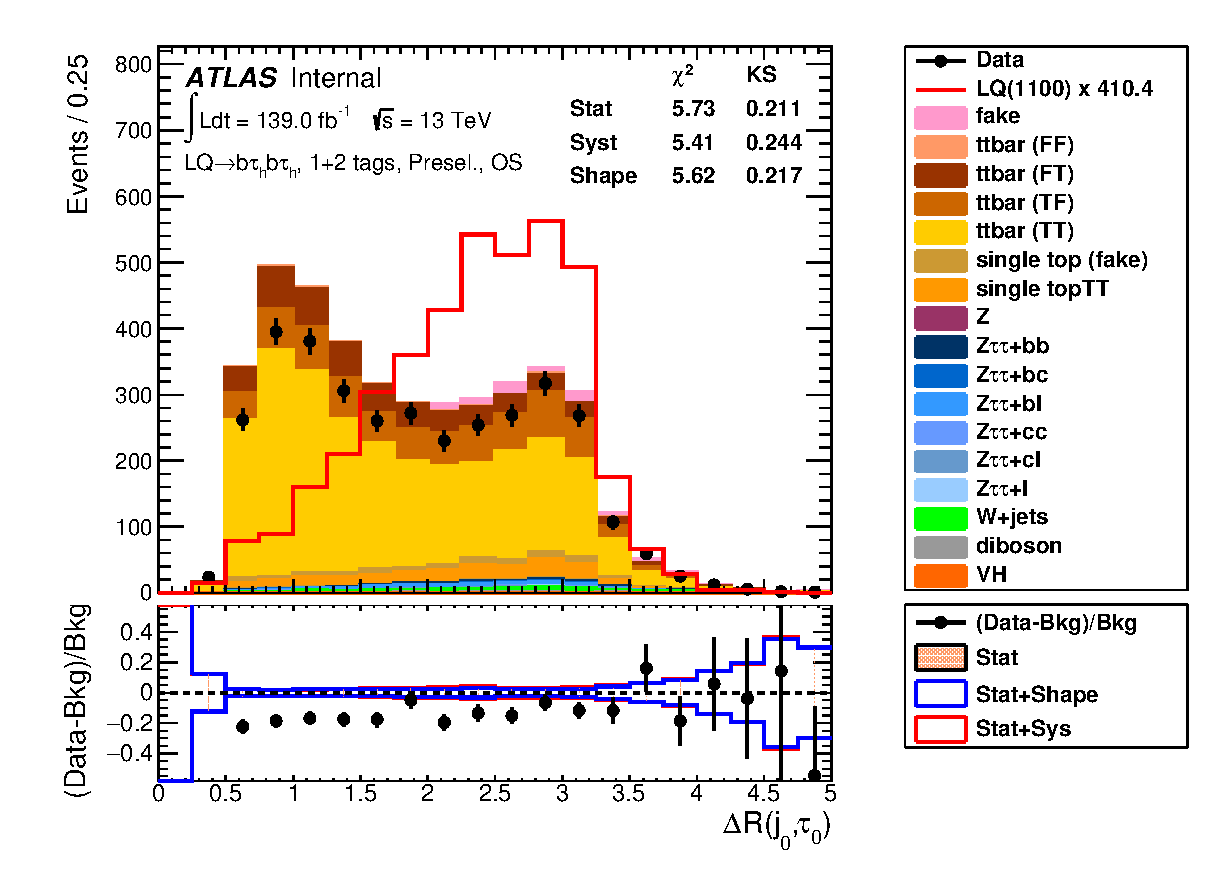
\includegraphics[width=0.4\textwidth]{figures/mva/lq3/hadhad/C_3tag2pjet_0ptv_OS_SR_DRTauJetLQ.eps}}
    \caption{ 
     The pre-fit PNN input variable distributions in the LQLQ \hadhad signal region. The red coloured line shows the LQ \hadhad signal yields ($m=1100$ GeV).
    }
     \label{fig:PNN_input_hadhad}
\end{figure}



\begin{figure}
    \centering
    \subfloat[]{ \includegraphics[width=0.4\textwidth]{figures/mva/lq3/hadhad/prefit_PNN/Region_BMin0_incJet1_dist500_J2_Y2015_DOSSRLQ3PNN0_T3_SpcTauHH_L0_Prefitlog.pdf}}
    \subfloat[]{ \includegraphics[width=0.4\textwidth]{figures/mva/lq3/hadhad/prefit_PNN/Region_BMin0_incJet1_dist800_J2_Y2015_DOSSRLQ3PNN0_T3_SpcTauHH_L0_Prefitlog.pdf}} \\
    \subfloat[]{ \includegraphics[width=0.4\textwidth]{figures/mva/lq3/hadhad/prefit_PNN/Region_BMin0_incJet1_dist1000_J2_Y2015_DOSSRLQ3PNN0_T3_SpcTauHH_L0_Prefitlog.pdf}}
    \subfloat[]{ \includegraphics[width=0.4\textwidth]{figures/mva/lq3/hadhad/prefit_PNN/Region_BMin0_incJet1_dist1200_J2_Y2015_DOSSRLQ3PNN0_T3_SpcTauHH_L0_Prefitlog.pdf}} \\
    \subfloat[]{ \includegraphics[width=0.4\textwidth]{figures/mva/lq3/hadhad/prefit_PNN/Region_BMin0_incJet1_dist1400_J2_Y2015_DOSSRLQ3PNN0_T3_SpcTauHH_L0_Prefitlog.pdf}}
    \subfloat[]{ \includegraphics[width=0.4\textwidth]{figures/mva/lq3/hadhad/prefit_PNN/Region_BMin0_incJet1_dist1600_J2_Y2015_DOSSRLQ3PNN0_T3_SpcTauHH_L0_Prefitlog.pdf}} \\
    \caption{ 
     The pre-fit PNN distributions in the LQLQ \hadhad signal region. The red coloured line shows the LQ \hadhad signal yields.
    }
     \label{fig:PNN_hadhad}
\end{figure}

\FloatBarrier
